% REMEMBER TO SET LANGUAGE!
\documentclass[a4paper,10pt,english]{article}
\usepackage[utf8]{inputenc}
\usepackage[norsk]{babel}
% Standard stuff
\usepackage{amsmath,graphicx,varioref,verbatim,amsfonts,geometry}
% colors in text
\usepackage[usenames,dvipsnames,svgnames,table]{xcolor}
% Hyper refs
\usepackage[colorlinks]{hyperref}

\usepackage{caption}
\usepackage{subcaption}
% Document formatting
\setlength{\parindent}{0mm}
\setlength{\parskip}{1.5mm}

%Color scheme for listings
\usepackage{textcomp}
\definecolor{listinggray}{gray}{0.9}
\definecolor{lbcolor}{rgb}{0.9,0.9,0.9}

%Listings configuration
\usepackage{listings}
%Hvis du bruker noe annet enn python, endre det her for å få riktig highlighting.
\lstset{
	backgroundcolor=\color{lbcolor},
	tabsize=4,
	rulecolor=,
	language=python,
        basicstyle=\scriptsize,
        upquote=true,
        aboveskip={1.5\baselineskip},
        columns=fixed,
	numbers=left,
        showstringspaces=false,
        extendedchars=true,
        breaklines=true,
        prebreak = \raisebox{0ex}[0ex][0ex]{\ensuremath{\hookleftarrow}},
        frame=single,
        showtabs=false,
        showspaces=false,
        showstringspaces=false,
        identifierstyle=\ttfamily,
        keywordstyle=\color[rgb]{0,0,1},
        commentstyle=\color[rgb]{0.133,0.545,0.133},
        stringstyle=\color[rgb]{0.627,0.126,0.941}
        }
        
\newcounter{subproject}
\renewcommand{\thesubproject}{\alph{subproject}}
\newenvironment{subproj}{
\begin{description}
\item[\refstepcounter{subproject}(\thesubproject)]
}{\end{description}}

%Lettering instead of numbering in different layers
%\renewcommand{\labelenumi}{\alph{enumi}}
%\renewcommand{\thesubsection}{\alph{subsection}}

%opening
\title{FYS-MEK1110 - Prosjektoppgave}
\author{Jens Tandstad}

\begin{document}

\maketitle
\newpage

\section*{1}
The Lennard Jones potential t is given by the function.
\begin{equation}
U(r) = 4\epsilon \left(   (\frac{\sigma}{r})^{12} -   (\frac{\sigma}{r})^6 \right)
\end{equation}

\subsection*{1a )i}
\textbf{Plot the potential as a function of r with $\epsilon$ = 1 and $\sigma$ = 1, for example for $r \in [0.9, 3]$}
\begin{figure}[h!]
        \centering 
        %Scale angir størrelsen på bildet. Bildefilen må ligge i samme mappe som tex-filen. 
        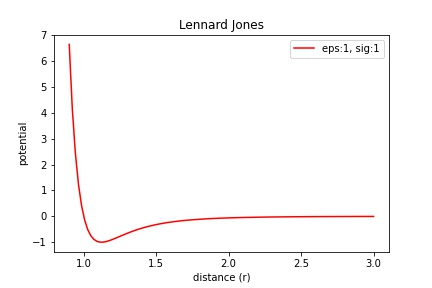
\includegraphics[scale=0.6]{1a_i.jpg} 
        \caption{Lennard Jones potential with $\epsilon = 1$ and $\sigma = 1$, }
        %Label gjør det enkelt å referere til ulike bilder.
        \label{fig:eksempelbilde1}
\end{figure}

\subsection*{1a )ii}
\textbf{The behaviour of U(r) is vastly different for $r < \sigma$ and $r > \sigma$. Which term in the potential, equation (1),
dominates in each case and what is the effect?}

The term in the twelfth power $\frac{\sigma}{r}^12$ dominates for $r < \sigma$ because the powered term is $ > 1$. The high power means the value of the first term blows up quickly. When $r < \sigma$, it will be quickly diminished. When $r = \sigma$ the two terms cancel out. The effect is that for values at distance where $r > \sigma$, there is an attractive force and for $r < \sigma$ a repelled force.

\subsection*{1a )iii}
\textbf{Find and characterise the equilibrium points of the potential.
}
The equillibrium points can be identified by looking at the graph and finding the lowest possible value. It can also be done by solving the equation.  The equillibrium poonit must be the value of $r$, where the bonding potential can only be increased by altering the distance, i.e the force acting on the particle must be at its minimum. This must be where the derivative of the potential is 0, which happens at approximately $r = 1.1\sigma$. 

We can also solve this by taking the derivative with respect to distance and setting it to zero.
\begin{equation}
\frac{\partial U(r)}{\partial r} = 0
\end{equation}

The derivation 
\begin{equation}
U(r) = 
4\epsilon \left(   (\sigma r^{-1})^{12} -   (\sigma r^{-1})^6 \right)  
\end{equation}

\begin{equation}
U(r) = 
4\epsilon \left(   \sigma^{12} r^{-12} -  n \sigma^{12} r^{-6} \right) 
\end{equation}


\begin{equation}
\frac{\partial U(r)}{\partial r} = 
4\epsilon \sigma^{12} \left(   -12  r^{-13} + 6 \cdot   r^{-7} \right)
\end{equation}

Simplifying we end up with
\begin{equation}
\frac{\partial U(r)}{\partial r} = 
4\epsilon \sigma \left( 2  r^{-13} -   r^{-7} \right) = 0
\end{equation}

Because $\sigma$ is a constant we can set to whatever,  we do not need to keep the $\sigma^{12}$. Also we focus on the inside of parenthesis, which must be equal to 0. Taking the lowest common denominator of the parenthesis, leaves leave us with:

\begin{equation}
2-r^6=0
\end{equation}

\begin{equation}
\sqrt[6]{2}= r
\end{equation}
The equillibrium point is given by 

\begin{equation}
4\epsilon \sigma \sqrt[6]{2}
\end{equation}




\subsection*{1a )iv}
\textbf{Describe qualitatively the motion of two atoms which start at rest separated by a distance of
$1.5\sigma$. What if they start with a separation of $0.95\sigma$? (Hint: use the graph of the potential.)}
The motion of two atoms starting at rest separated by distance of *$1.5 \sigma$ (i.e if the $\sigma$ is 1, then $r = 1.5$  will be subject to a weak negative gradient. This attraction will grow until it reaches the maximum bonding potential at around radius of $r = 1.1 \sigma$.
If the particles in stead start at 0.95, they will move away from one another and again stabilize at the same point of maximum bonding potential.

\subsection*{1a )v}
\textbf{Describe the shape of the potential close to the stable equilibrium point. Can you think of other
force(s) with the same behaviour?}

Around the point of maximum bonding potential, the potential can be approximated by a parabolic equation, such as $x^2$. There are other forces that act in this way, including the weak and the strong nuclear force.

\section*{1b) i}
\textbf{Find the force on atom $i$ at position $\vec{r}_i$
from atom $j$ at position $\vec{r}-j$}

We can replace the radius $r$ in previous equation, with the length of the vector between the two particles. The  force acting atom $i$ at position $\vec{r_i}$ from atom $j$ at position $r_j$ must then be. 

\begin{equation}
U(r) = 4\epsilon \left(   (\frac{\sigma}{|| r_i - r_j || })^{12} -   (\frac{\sigma}{|| r_i - r_j || })^6 \right)
\end{equation}

\subsection*{ii}
\textbf{Show that the equation of motion for atom i is...}

The equation of motion, is given by the differential equation:

\begin{equation}
\vec{r}_{i+1} = r_{i} \cdot \frac{\partial r_{i}}{\partial t}
\end{equation}

We intuitively understand that the term $\frac{d r_{i}}{d t}$, change in position is the same as velocity, i.e the speed at which the particles are travelling. 

The Lennard Jones potential describes the forcs  acting on a particle. These forces accelerate the particle in a particular direction. This acceleration affects velocity, which in turn affects position. In the same manner as above, we can write the equation of velocity at time $t$ as the differential equation:

\begin{equation}
\vec{v}_{i+1} = v_{i} \cdot \frac{d v_{i}}{d t}
\end{equation}

The acceleration is given by the change in the potential. The intuition is that if an atom is within the potential somewhere, the force that will be acting on it is the difference between the force acting on one side, and the other side. This must be equal to the rate of change of the potential, i.e the derivative of the potential.

The term $\frac{\partial v_{i}}{\partial t}$ is here obviously the acceleration. We have these three names for the equation of \textbf{acceleration}.

\begin{equation}
 \frac{d^2 \vec{r_i}}{dt^2} =  \frac{d v_{i}}{d t}   = \vec{a}_i
\end{equation}

Let the force F be the attractive force of the potential, as a function of the distance. It is negative because the potential is attractive.
\begin{equation}
F = -U'(d)
\end{equation}

Deriving the Lennard Jones potential gives us

\begin{equation}
U'(d) = 4\epsilon \left( -12  (\frac{\sigma^{12}}{d^{13}}) + 6 (\frac{\sigma^6}{d^7 } \right)
\end{equation}

This can be simplified to :

\begin{equation}
U'(d) = -24\epsilon \left( -2  (\frac{\sigma^{12}}{d^{13}}) + (\frac{\sigma^6}{d^7 } \right)
\end{equation}

Which transforms to:

\begin{equation}
-U'(d) = 24\epsilon \left( 2  (\frac{\sigma^{12}}{d^{13}}) - (\frac{\sigma^6}{d^7 } \right)
\label{eq:derivedPotential}
\end{equation}


This equation applies to each particles interaction with a second particle. There are $n^2$ such relations, pushing and pulling in different directions in 3D space. To properly apply this force in 3D space, we must multiply the force by the force by the unit vector pointing from the $i$-th to the $j$-th particle. This yields an acceleration vector $\vec{a_{i+1}}$ acting between particles $i$ and $j$ at a point in time. By summing these vectors over all other particles, we get the net force acting on the particle at a point $t$:

\begin{equation}
\vec{a_{i+1}} =   \sum_{j \neq i}  \left(  F(||\vec{r_i} - \vec{r_j} ||) \right)( |\vec{r_i} - \vec{r_j} |)
\label{eq:sumPotential}
\end{equation}

Note that the $j \neq i$ avoid the particle interacting with itself.

We now insert the equation from \eqref{eq:derivedPotential} into \eqref{eq:sumPotential}, and replace $d$ with $||\vec{r_i} - \vec{r_j} ||$.


\begin{equation}
\vec{a_{i+1}} =   \sum_{j \neq i}  \left(  
24\epsilon \left( 2  (\frac{\sigma^{12}}{(||\vec{r_i} - \vec{r_j} ||)^{13}}) 
- (\frac{\sigma^6}{(||\vec{r_i} - \vec{r_j} ||)^7 } \right)\right)|\vec{r_i} - \vec{r_j} |
\label{eq:sumPotential}
\end{equation}

Almost there.  The last term - the normalized  unit vector $|\vec{r_i} - \vec{r_j} |$ , can also be written as the distance vector divided by its length:

\begin{equation}
|\vec{r_i} - \vec{r_j} | = \frac{ \vec{r_i} - \vec{r_j} }{ ||\vec{r_i} - \vec{r_j} ||}
\end{equation}
We will replace the last term with this. Also notice that the denominator is set to the 13th and 7th power. We can subtract one here, by squaring the denominator in the final term. This allows us to combine the powers inside the equation again, and avoid having different powers on the numerator and denominator. We have:

\begin{equation}
\vec{a_i} = \frac{d^2 r_i}{dt^2} =   \sum_{j \neq i} 24\epsilon \left( 2 (\frac{\sigma}{|| r_i - r_j||})^{12} -  (\frac{\sigma}{|| r_i - r_j||})^6 \right)(\frac{ \vec{r_i} - \vec{r_j} }{ ||\vec{r_i} - \vec{r_j} ||^2})
\end{equation}


\subsection*{1c)}

\subsection{1c) i}
\textbf{Introduce the scaled coordinates $\vec{r_i}'= \frac{\vec{r_i}}{\sigma}$ and show that the equation of motion can be rewritten in terms of these coordinates as}

Using reduced units, this simplifies equations considerably. First We modify the acceleration equation so that the distance between atoms is measured in sigmas $\sigma$. 

\begin{equation}
\vec{a_i}  =  \frac{d^2 r_i}{dt^2}  =  \sum_{j \neq i} 24 \epsilon \sigma \left(   ( 2 || r_i - r_j ||)^{-12} -   ((|| r_i - r_j ||)^{-6} \right)(\frac{ \vec{r_i} - \vec{r_j} }{ ||\vec{r_i} - \vec{r_j} ||})
\end{equation}

Because $\epsilon$ and $\sigma$ are scalars, there must an inverse scalar to each, such such that  $\sigma \sigma=^{-1} 1$. Scaling the equation using this his allows us to set $\epsilon$ and $\sigma$ to 1, yielding:
\begin{equation}
 \frac{d^2 r_i'}{dt'^2}  =  \sum_{j \neq i} 24  \left(   ( 2 || r_i' - r_j' ||)^{-12} -   ((|| r_i' - r_j' ||)^{-6} \right)(\frac{ \vec{r_i}' - \vec{r_j}' }{ ||\vec{r_i}' - \vec{r_j}' ||})
\end{equation}

We removed $\epsilon$ and mass $m$ from the equation, by setting both to 1. 


\subsection*{1c) ii}

With reduced units we lose track of the the actual distances, speeds. We obtain however, a general solution for many different gases which means we can use one simulation for many types of gases. We can get the velocities,  temperature, distance in meters etc by multiplying this general reduced result with an Atom specific set of numbers. $\sigma$ gives us the distances, but what about speeds? For that we need at unit that transforms our reduced time $t'$ to seconds.

There must be a scalar $\tau$, which transforms the velocity in sigma to velocity in meters per second. This relation is obviously affected by the units which the mass and energy is given in. If the units are given in pounds, $\tau$ must be different than if the units are given in metric system. By the magic of the SI unit system, this relation turns out to be the square of the \textbf{weight} of the atom (in kg)  divided by its \textbf{energy} in Electron-Volts.

\begin{equation}
\tau = \sqrt{\frac{m}{\epsilon}} = \sqrt{\frac{39.95 \cdot 1.66 \cdot 10^{-27} kg}{1.0318 \cdot 10^2 eV} }.
\end{equation}

This allows us to convert velocities measured in $\sigma$ to metric units by multiplying our time with $\tau$. 


The charateristic time-scale 
\begin{equation}
\tau = \sqrt{2.93686E-11 s}
\end{equation}




\newpage

\section*{Two atom simulations 2a)}
\subsection*{i}
\textbf{Write a function which solves equation (3) for two atoms and finds the positions and velocities
of the atoms as a function of time. Implement three different integration methods: Euler,
Euler-Cromer and Velocity-Verlet (see appendix C on page 11 for a description of the latter)}
We have created the Euler, EulerCromer and Velocity verlet algorithms. See appendix A for the kode. 

\section*{2b)}

\subsection*{2b) i)}
\textbf{. Simulate the motion of two atoms which start at rest separated by a distance of $1.5\sigma$ Use $\delta t  = 0.01$, simulate until $t
0 = 5$ and integrate with the Euler-Cromer method.}

\subsection*{2b) ii)}
\textbf{Plot the distance between the atoms as a function of time.}
We place two particles, one at origo and the other at positon  $(1.5\sigma, 0, 0)$. We therefore expect motion to be only happening on the x-axis. Using $\delta t$ of $0.01$, for $T = 5$. We simulate using Euler Cromer.

We plot the distance between the two particles in Figure (\ref{fig:two-particle-distance-15}).
\begin{figure}[h!]
        \centering 
        %Scale angir størrelsen på bildet. Bildefilen må ligge i samme mappe som tex-filen. 
        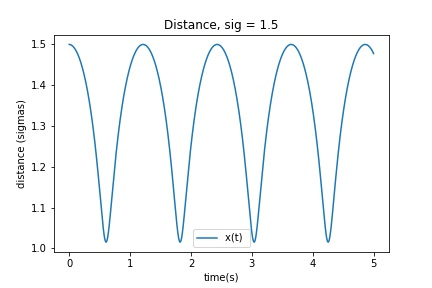
\includegraphics[scale=0.8]{./py/two-particle-distance-15.jpg} 
        \caption{Argon distance  with $D = 1.5 \sigma, \epsilon = 1$ and $\sigma = 1$, }
        %Label gjør det enkelt å referere til ulike bilder.
        \label{fig:two-particle-distance-15}
\end{figure}

\subsection*{2b) iii)}
\textbf{How does the motion fit with your expectations from exercise 1a) on the preceding page?}
Due to the potential not being symmetric, the expectation was that the particles would move more slowly toward each other than apart. We can see that the particles are being pulled toward each other constantly. 

\subsection*{iv)}
\textbf{Repeat the previous tasks, but now with an initial separation of $0.95 \sigma$. Explain your results}
In this second experiment, the two atoms are positioned closer, and within the region where the repulsive force dominates. Figure  (\ref{fig:two-particle-distance-095} shows how their distance increases rapidly. Because the repulsive energy is so much stronger than the attractive, a distance of $0.95\sigma$ we re in the repulsive range of the Lennard Jones potential. This accellerates the particles away from each other strongly enough that the particles eventually escape the attraction between particles and continue in opposite direcitons. 

\begin{figure}[h!]
        \centering 
        %Scale angir størrelsen på bildet. Bildefilen må ligge i samme mappe som tex-filen. 
        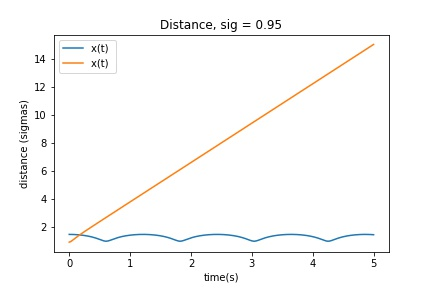
\includegraphics[scale=0.8]{./py/two-particle-distance-095.jpg} 
        \caption{Argon distance with $D = 0.95 \sigma, \epsilon = 1$ and $\sigma = 1$ }
        %Label gjør det enkelt å referere til ulike bilder.
        \label{fig:two-particle-distance-095}
\end{figure}


\newpage
\section*{2c}


\subsection*{2c) i)}
 \textbf{Plot the kinetic, potential and total energy as a function of time for the two cases in the previous
section}

Plotting the total energy in Figure \ref{fig:allEnergies}.

\begin{figure}[h!]
        \centering 
        %Scale angir størrelsen på bildet. Bildefilen må ligge i samme mappe som tex-filen. 
        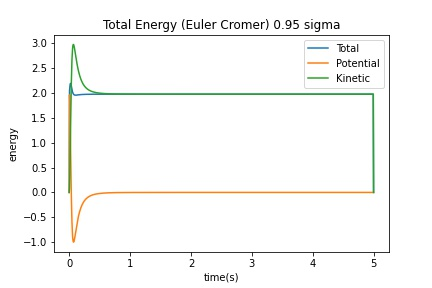
\includegraphics[scale=0.8]{./py/2ci_allEnergiesCromer15.jpg} 
        \caption{Euler Cromer method : Argon distance with $D = 1.5 \sigma, \epsilon = 1$ and $\sigma = 1$ }
        %Label gjør det enkelt å referere til ulike bilder.
        \label{fig:allEnergiesEuler15}
\end{figure}


\begin{figure}[h!]
        \centering 
        %Scale angir størrelsen på bildet. Bildefilen må ligge i samme mappe som tex-filen. 
        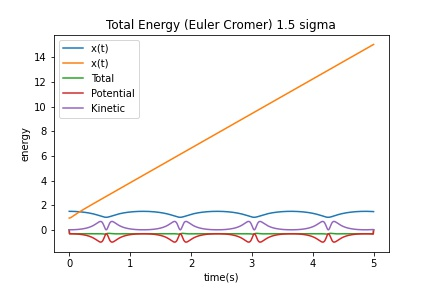
\includegraphics[scale=0.8]{./py/2ci_allEnergiesCromer095.jpg} 
        \caption{Euler cromer method : Argon distance with $D = 0.95 \sigma, \epsilon = 1$ and $\sigma = 1$ }
        %Label gjør det enkelt å referere til ulike bilder.
        \label{fig:allEnergiesEuler95}
\end{figure}


\subsection*{2c ) ii)}
\textbf{Theoretically speaking, should the total energy be conserved? Why, or why not? What about
momentum?
}

In theory, the energy should be conserved. Whenever two particles get into contact with each other, they will affect each other in a similar amount, but in opposite directions. As a result, kinetic energy will be conserved. As the potential energy is 0 when they are far away, there is no force acting on the particles.


\subsection*{2c ) iii)}
\textbf{How does the motion fit with your expectations from exercise 1a) on the preceding page?}
It fits exactly. Judging from the graphs, total energy is conserved in all the methods. . Kinetic energy is the velocity vector multiplied by the mass, potential energy is the sum of the acceleration force. TODO (What is potential energy, and is the kinetic energy really velocity vector multiplied by mass constant? What about sigma?


\subsection*{2c iv)}
\textbf{Simulate the same system as in exercise 2b) on the previous page with the Euler, Euler-Cromer
and Velocity Verlet algorithms, and compare graphs of the total energy as a function of time.}


When looking at figures \ref{fig:allEnergiesEuler15} to \ref{fig:allEnergiesVerlet95}, we see that the three methods have quite different charts for total energy. Velocity Verlet stabilizes at energy 5.6, Euler Cromer around 4.3 and Euler close to 6 in total Energy. It's unclear why there is such a large difference in integration methods. The fact that the total energy stabilizes indicates that there is no energy leak. Ideally, the blue line (total energy) should be flat.

\begin{figure}[h!]
        \centering 
        %Scale angir størrelsen på bildet. Bildefilen må ligge i samme mappe som tex-filen. 
        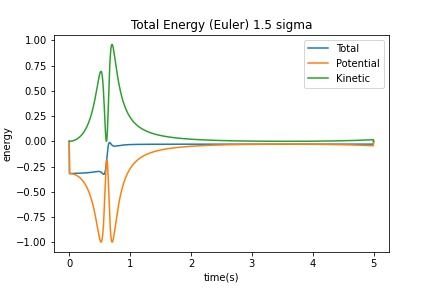
\includegraphics[scale=0.8]{./py/2civ_allEnergiesEuler15.jpg} 
        \caption{Euler method : Argon distance with $D = 1.5 \sigma, \epsilon = 1$ and $\sigma = 1$ }
        %Label gjør det enkelt å referere til ulike bilder.
        \label{fig:allEnergiesEuler15}
\end{figure}

\begin{figure}[h!]
        \centering 
        %Scale angir størrelsen på bildet. Bildefilen må ligge i samme mappe som tex-filen. 
        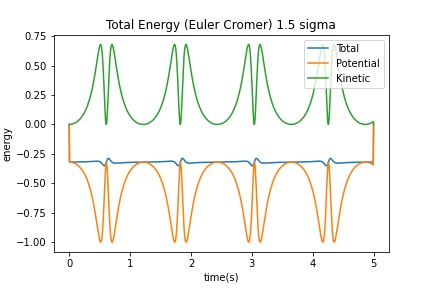
\includegraphics[scale=0.8]{./py/2civ_allEnergiesEulerCromer15.jpg} 
        \caption{Euler method : Argon distance with $D = 1.5 \sigma, \epsilon = 1$ and $\sigma = 1$ }
        %Label gjør det enkelt å referere til ulike bilder.
        \label{fig:allEnergiesEulerCromer15}
\end{figure}
\begin{figure}[h!]
        \centering 
        %Scale angir størrelsen på bildet. Bildefilen må ligge i samme mappe som tex-filen. 
        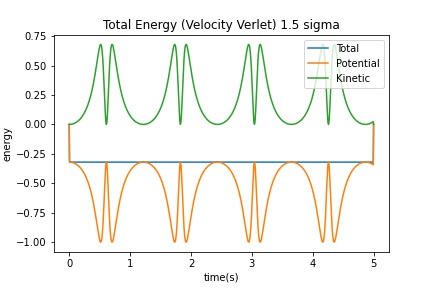
\includegraphics[scale=0.8]{./py/2civ_allEnergiesVelocityVerlet15.jpg} 
        \caption{Euler method : Argon distance with $D = 1.5 \sigma, \epsilon = 1$ and $\sigma = 1$ }
        %Label gjør det enkelt å referere til ulike bilder.
        \label{fig:allEnergiesVelver15}
\end{figure}

\begin{figure}[h!]
        \centering 
        %Scale angir størrelsen på bildet. Bildefilen må ligge i samme mappe som tex-filen. 
        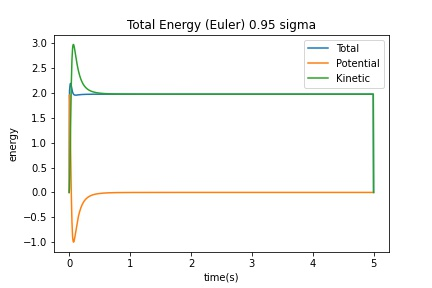
\includegraphics[scale=0.8]{./py/2civ_allEnergiesEuler095.jpg} 
        \caption{Euler  method : Argon distance with $D = 0.95 \sigma, \epsilon = 1$ and $\sigma = 1$ }
        %Label gjør det enkelt å referere til ulike bilder.
        \label{fig:allEuler95}
\end{figure}


\begin{figure}[h!]
        \centering 
        %Scale angir størrelsen på bildet. Bildefilen må ligge i samme mappe som tex-filen. 
        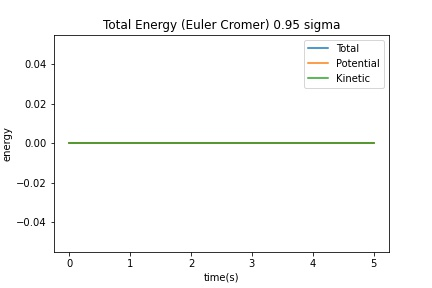
\includegraphics[scale=0.8]{./py/2civ_allEnergiesEulerCromer095.jpg} 
        \caption{Euler Cromer  method : Argon distance with $D = 0.95 \sigma, \epsilon = 1$ and $\sigma = 1$ }
        %Label gjør det enkelt å referere til ulike bilder.
        \label{fig:allEulerCromer95}
\end{figure}


\begin{figure}[h!]
        \centering 
        %Scale angir størrelsen på bildet. Bildefilen må ligge i samme mappe som tex-filen. 
        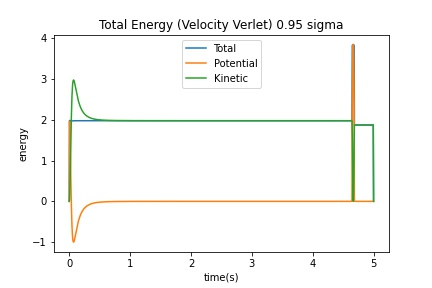
\includegraphics[scale=0.8]{./py/2civ_allEnergiesVelocityVerlet095.jpg} 
        \caption{Velocity verlet  method : Argon distance with $D = 0.95 \sigma, \epsilon = 1$ and $\sigma = 1$ }
        %Label gjør det enkelt å referere til ulike bilder.
        \label{fig:allEnergiesVerlet95}
\end{figure}





\subsection*{2c) v)}
\textbf{Find the largest time step that keeps stable motion and conserves energy for all three methods
(small fluctuations in energy are allowed as long as they are periodic and don’t increase/decrease
with time). Discuss your results.
}

When we experiment, we see that at a delta of $0.1$, the accuracy allows the particles to tunnel through each other to the other side. At half this, the graphs look pretty much the same except they are more pointy. With such low resolution graphs, it can be expected to be enough inaccuracy so that the simulation can be wrong.
The EulerCromer and Velocity Verlet are more resistant to higher delta t.

\subsection*{2c) vi)}
\textbf{Link your experimentation to a brief discussion of the pros and cons of the three methods, both
physically and computationally}

What method is a question of simplicity, accuracy and computational cost the $\delta t$.  The higher computational cost, the more accuracy is required for the algorithm to be viable. By including the second derivative, such as the acceleration, the Velocity Verlet approximates the change in the velocity using - basically - a second order Taylor polynomial. This additional complexity inside the algorithm, allowing it to "look ahead" and predict changes to the acceleration and velocity, allows a significantly longer $\delta t$. This might be enough to defend the computational cost of adding more terms, and so the algorithm might emerge faster on average.

However, the more complex an algorithm is, the more difficult it is to write and understand, and debug. If an agorithm is 10\% more effective, and takes 10 more hours to write and debug, the algorithm must run for at least 100 hours to recoup the loss on a machine with the same cost-basis as the developer. Usually, computing speed is less expensive than developer time, so its often much worse.

\subsection*{2d) i}
\textbf{. Extend your implementation such that it writes to an xyz-file at each timestep (see appendix A on page 11).}

The implementation writes to an xyz file, which can be opened by Ovito.

\subsection*{2d) ii}
\textbf{Visualise the results of your simulations using Ovito (see appendix B on page 11)}


\begin{figure}[h!]
        \centering 
        %Scale angir størrelsen på bildet. Bildefilen må ligge i samme mappe som tex-filen. 
        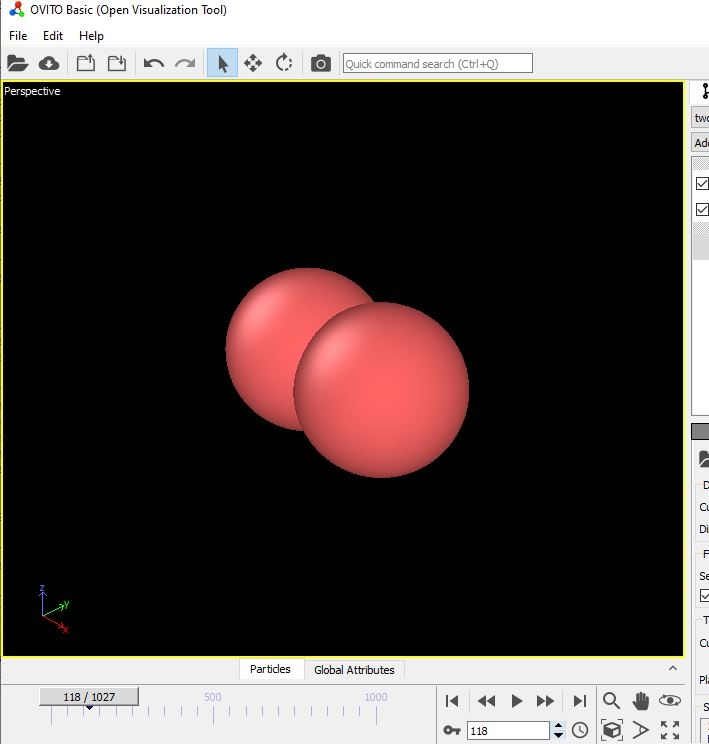
\includegraphics[scale=0.6]{./py/2dii_ovito.JPG} 
        \caption{Two atoms at distance $1.5 \sigma $ visualized in Ovito }
        %Label gjør det enkelt å referere til ulike bilder.
        \label{fig:2dii_ovito}
\end{figure}

\newpage

\section*{Part 3}

\subsection*{a) i}
\textbf{Implement a solver of equation (3) on the preceding page for N atoms, given initial positions
and velocities.
}
This was taken care of from the start, no changes needed.

\subsection*{a) ii}
\textbf{Use Newton’s third law to reduce the number of force calculations.
}
Newtons third law states that if a particle A exerts a force on another particle B, there must be an equal force acting in the other direction. We can take advantage of this by completing $A \rightarrow B$ when we have calculated $B \rightarrow A$.

In practise this means taking the cartesian product of all the particles , ignoring the diagonal (because A does not exert a force on itself.) In practise we only need to consider what is above and to the right of the diagonal.

In the code this has been implemented in the VelocityVerletFast algorithm. 


\subsection*{a) iii}
\textbf{Extend your implementation such that atoms more than $3\sigma$ apart do not interact}
The velocityVerletFast implementation also ignores particles that are more than $3 \sigma$ distance. It takes advantage of the fact that a cartesian matrix is mirrored around the diagonal. Therefore we can both ignore the diagonal (particles do not self-interact) and use only the upper triangle.


\subsection*{iv}
\textbf{Plot the shifted potential and the corresponding force to verify your implementation of the
cut-off.}

The shifted potential ensures that the force is a little weaker than the Lennard Jones potential. Because the LJ potential is itself an approximation, its ok to tinker with it a little bit. The benefit of a shifted potential is that there is a continous progression close to $3 \sigma $ and beyond it.

\begin{figure}[h!]
        \centering 
        %Scale angir størrelsen på bildet. Bildefilen må ligge i samme mappe som tex-filen. 
        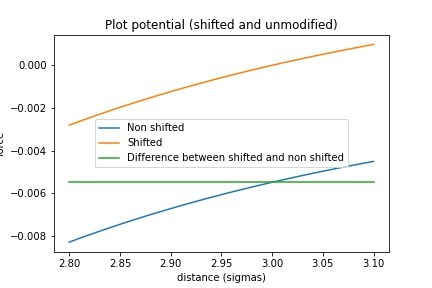
\includegraphics[scale=0.6]{./py/plotPotentialDiff.jpg} 
        \caption{Shifted  Lennard Jones  potential becomes 0 at exactly $3\sigma$, allows cutoff at this range }
        %Label gjør det enkelt å referere til ulike bilder.
        \label{fig:eksempelbilde1}
\end{figure}

\subsection*{a) v}
\textbf{Does the shift of the potential described above impact the force calculations?}
Because the potential is a constant, it does not affect the derivative, i.e the slope of the curve. The force is simply set to zero a little earlier. This makes any effects of the attractive force at distances greater than the cutoff length nil. This could obviously be bad, but in most cases there is a range in which this doesn't matter, either because it's too weak, or because it is crowded out by many more and stronger attractions from closer particles. The shift also makes the repulsive force kick in a little bit sooner. This part of the potential is so steep anyway that it doesn't make a difference in practise. 

Note that the shifted potential doesn't affect how the particles are accelerated, when in range. It only shifts the position slightly when they are affected.


\subsection*{3b) i}
\textbf{Reproduce your results for the 2-atom model from the previous section to verify your implementation.}

Comparing the xyz files produces by the optimized VelocityVerlet and the non-optimised gives results that are indistinguishable upon inspection.

\subsection*{3b) ii}
\textbf{Simulate the motion of four atoms starting at rest from the positions}
This was been done.

\subsection*{3b) iii}
\textbf{Visualise the results in Ovito, describe and explain the motion.}

The atoms remain in a steady state, perfectly positioned in a square. They move inwards and outwards slowly, and but being pulled toward the through in the potential. The reason is that the starting distance is very close to the distance of the the through.


\begin{figure}[h!]
        \centering 
        %Scale angir størrelsen på bildet. Bildefilen må ligge i samme mappe som tex-filen. 
        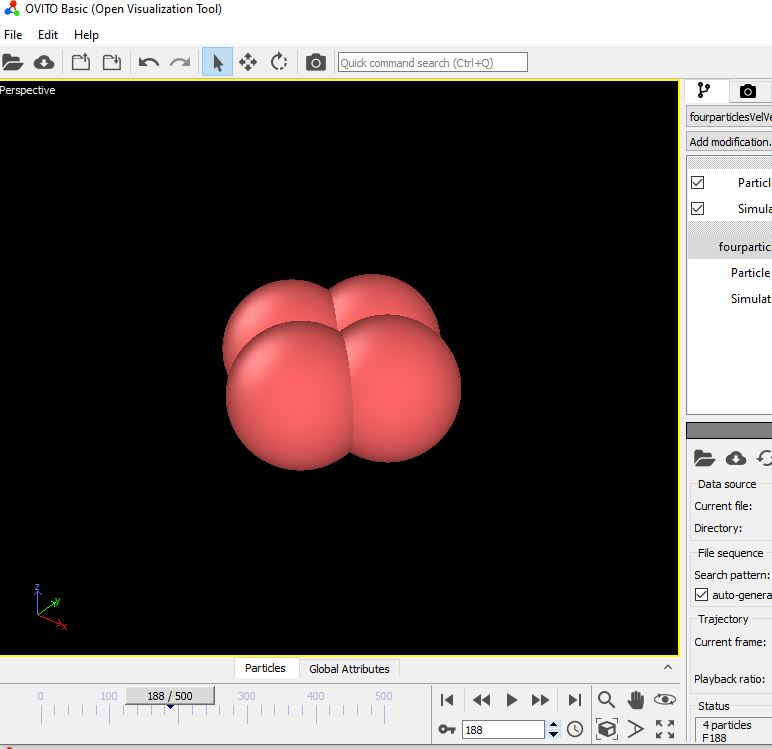
\includegraphics[scale=0.6]{./py/3biii_ovito.jpg} 
        \caption{Four particles visualised in Ovito}
        %Label gjør det enkelt å referere til ulike bilder.
        \label{fig:3biii}
\end{figure}


\subsection*{3b)iv}
\textbf{Plot the potential, kinetic and total energy as a function of time, and comment on the energy
conservation}

We plot the energies, and see that there are no runaway accumulation or leak. The energy is conserved.

\begin{figure}[h!]
        \centering 
        %Scale angir størrelsen på bildet. Bildefilen må ligge i samme mappe som tex-filen. 
        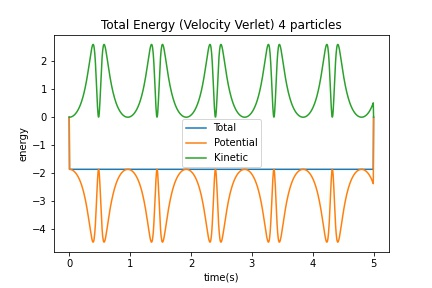
\includegraphics[scale=0.6]{./py/3b_iv.jpg} 
        \caption{256 atoms energy}
        %Label gjør det enkelt å referere til ulike bilder.
        \label{fig:3biv}
\end{figure}

\subsection*{3b)v}
\textbf{Repeat the above exercises with a small perturbation in the initial positions, such that the first
atom starts at}
We repeat it with a small perturbation, ans immediately see a large amount of randomness emerge. The introduction of the perturbation makes the movement chaotic, and it becomes much harder to tell if there is a leak. It's therefore a good idea to check the integrity of energy conservation using simpler setups.


\begin{figure}[h!]
        \centering 
        %Scale angir størrelsen på bildet. Bildefilen må ligge i samme mappe som tex-filen. 
        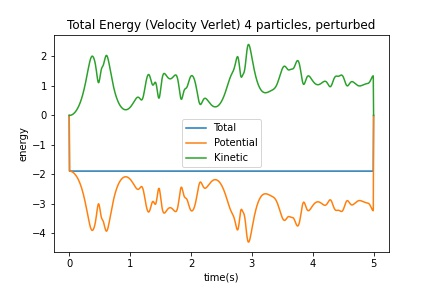
\includegraphics[scale=0.6]{./py/3b_v.jpg} 
        \caption{Total energy between four atoms }
        %Label gjør det enkelt å referere til ulike bilder.
        \label{fig:3biv}
\end{figure}

\subsection*{3c) i}
\textbf{Write a function which takes n and L (or n and d) as arguments and returns the positions of 4n
3
atoms on a face-centred cubic lattice.
}

I have made a function in the  \textbf{MDGennerators} modules, named \textbf{PopulateCreateCrystalStructure}(3, 1). This takes as an argument the number of unit cells and the distance between them. Each cell contains four tetrahedrally placed Argon atoms.

\subsection*{3c) ii}
\textbf{Verify your implementation by calling your function for n = 3 and L = 20, writing the resulting
positions to an xyz-file and looking at the result in Ovito. Your system should contain 4 · 3
3 = 108
atoms.}

Verifying that there are 108 particles in the crytal.

\subsection*{3c) iii}
\textbf{Show that the unit cell size corresponding to the density $\rho = 1.374 g/cm3$
is $d = 1.7\sigma$ This will be used in the remaining parts of the project.}

Reasoning : The unit cell size corresponding to 1.374 g per $cm^3$ must be equal to the mass of the atom Argon, multiplied with the number of particles that fit within 1 $cm^3$.

In order for the mass to be 1.375 grams per cubic centimeter, the number of unit cells containing four atoms in one centimeter must be known, and the mass of each atom must be known. 


\begin{equation}
4m \cdot  n^3 = 1.375 g/cm^3
\end{equation}

The distance for  $\sigma $ that is associated with this density, we name $\sigma_d$, and it can be expressed as the $1 cm / n$. Hence, converting the centimeter to meters units, $\sigma_d$ must be given by :


\begin{equation}
\sigma_d= \frac{0.01}{n}
\end{equation}

We were told that the value for $\sigma$ for Argon was $3.405Å$. Hence, our value for $\sigma_d$ should be exactly $3.405 \cdot 1.7 Å$.Expected value for $\sigma_d = 3.405 \cdot 1.7 = 5.7885 Å$

We must now find the value for $n$. , 
\begin{equation}
4m \cdot  n^3 = \frac{1.375 g}{1 cm^3} 
\end{equation}


We were given the mass $m$ of Argon as $m = 39.95 u, u = 1.66 \cdot 10^{-27}g$, which is then 

\begin{equation}
39.95 \cdot 1.66 \cdot 10^{-27} = 6.6317E-26 g 
\end{equation}

This equation then gives us

\begin{equation}
4(6.6317 \cdot 10^{-26} g ) \cdot  n^3 = \frac{1.375 g}{1 cm^3}
\end{equation}

Solving this for $n$ using tools should give us the number of unit squares per cm.

\begin{equation}
n =\sqrt[3]{\frac{5^{26}\cdot \:23068672}{6.6317}} = 173063684.30366
\end{equation}

Dividing this cm into 173063684.30366 units, and converting the distance to Ångstrøm units,  gives us:

\begin{equation}
\sigma_d = \frac{1}{173063684.30366} \cdot  10^{9} = 5.778219 Å
\end{equation}


When multiplying to get the size in Ångstrøms, we multiply with $10^9$, because this is 10 magnitudes increase from 1, the initial 10. This is another 9 magnitudes. This shows that we get the same value as expected. We have thus connected the mass of the molecule, distance between unit cells $\sigma$ and the density.

We will now use the $\sigma_d = 1.7 $ for the remainder of the project.



\subsection*{3d) ii}
\textbf{Simulate 256 atoms starting from rest, and visualise the result}

I have simulated with 256 atoms, creating this crystal structure

\begin{figure}[h!]
        \centering 
        %Scale angir størrelsen på bildet. Bildefilen må ligge i samme mappe som tex-filen. 
        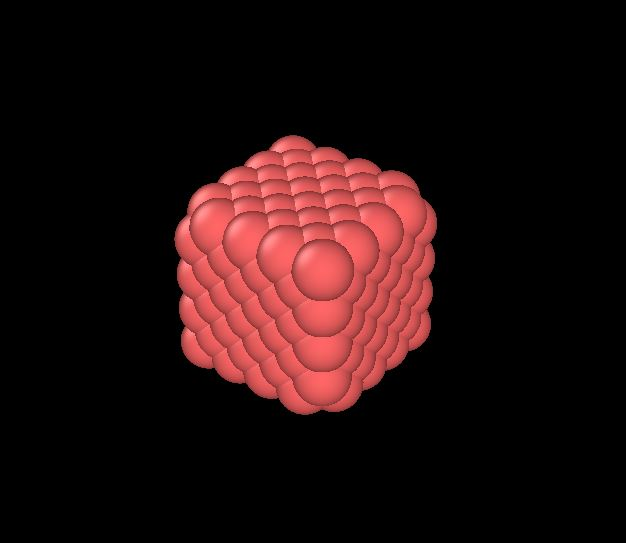
\includegraphics[scale=0.6]{./py/3di_1_ovito.jpg} 
        \caption{Crystal lattice }
        %Label gjør det enkelt å referere til ulike bilder.
        \label{fig:3di_1}
\end{figure}


\subsection*{3d) ii}
\textbf{Plot the potential, kinetic and total energy as a function of time. What is the main difference
from the energy graphs for two and four atoms?
}

The difference is apparent. The more atoms, the more forces are acting between the particles. The net result is that variations in positions are smaller. This can also be interpreted as higher number of close particles, means higher probability of interacting with those particles.

\begin{figure}[h!]
        \centering 
        %Scale angir størrelsen på bildet. Bildefilen må ligge i samme mappe som tex-filen. 
        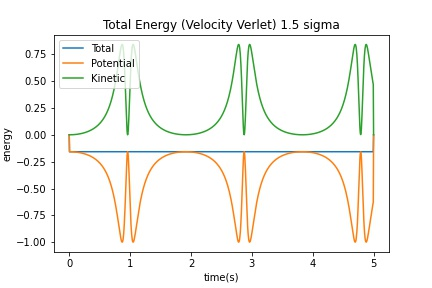
\includegraphics[scale=0.6]{./py/3dii_energy_two.jpg} 
        \caption{Energy for two atoms}
        %Label gjør det enkelt å referere til ulike bilder.
        \label{fig:3di_2}
\end{figure}
\begin{figure}[h!]
        \centering 
        %Scale angir størrelsen på bildet. Bildefilen må ligge i samme mappe som tex-filen. 
        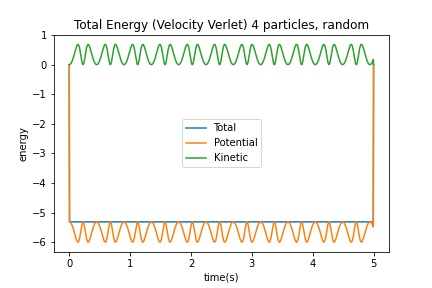
\includegraphics[scale=0.6]{./py/3dii_energy_four.jpg} 
        \caption{Energy for four atoms}
        %Label gjør det enkelt å referere til ulike bilder.
        \label{fig:3di_2}
\end{figure}


\newpage
\subsection*{3e) i}
\textbf{Implement either periodic or reflective boundary conditions (or both) in your program}

I have implemented both, but it was actually easier to get the periodic to work. 



\subsection*{3e) ii}
 \textbf{Run a simulation with 108 atoms and verify visually that your implementation works. Give the
atoms some initial velocities of your own choosing.}

I have used the Crystal populating function, and created the atoms.


\begin{figure}[h!]
        \centering 
        %Scale angir størrelsen på bildet. Bildefilen må ligge i samme mappe som tex-filen. 
        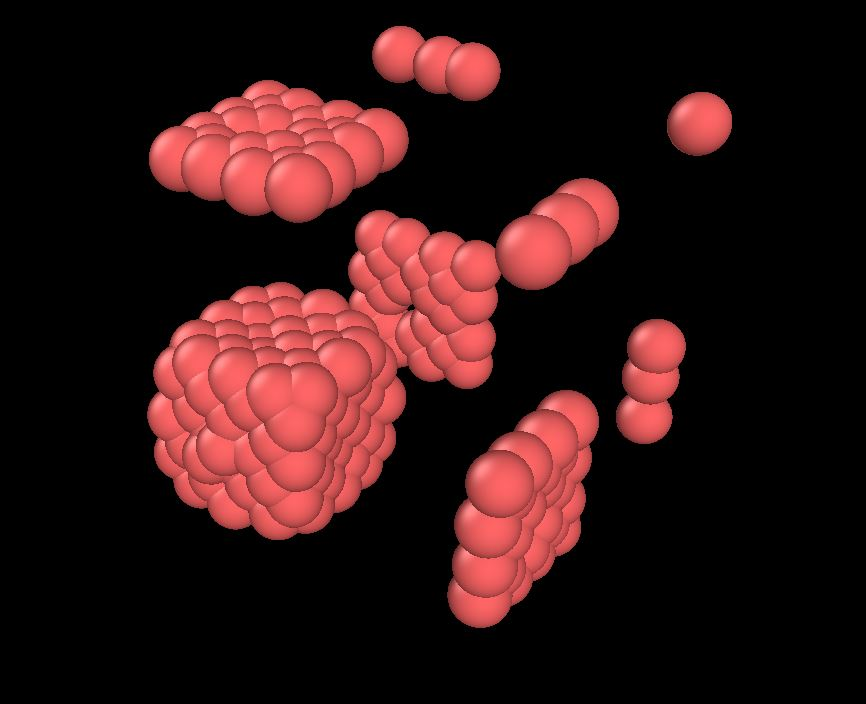
\includegraphics[scale=0.6]{./py/3di_3_ovito.jpg} 
        \caption{Periodic boundary conditions apparent}
        %Label gjør det enkelt å referere til ulike bilder.
        \label{fig:3di_2}
\end{figure}


\begin{figure}[h!]
        \centering 
        %Scale angir størrelsen på bildet. Bildefilen må ligge i samme mappe som tex-filen. 
        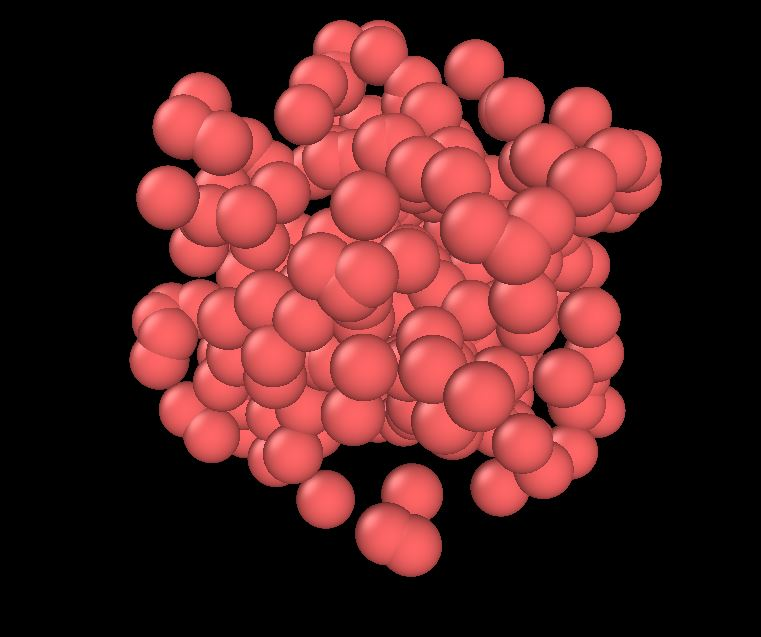
\includegraphics[scale=0.6]{./py/3di_2_ovito.jpg} 
        \caption{Crystal has expanded to fill box}
        %Label gjør det enkelt å referere til ulike bilder.
        \label{fig:3di_2}
\end{figure}



\newpage


\section*{4. Science}
\subsection*{4a)  i }
\textbf{ Extend your implementation with the calculation of temperature.
}

I have added the function plotTemperature to the file MDPlot.  This depends on the \textbf{ComputeTemperatureReduced} function, which essentially converts the kinetic energy (squared) to Kelvin.

It used the reduced form equation, and then converts to Kelving afterwards. N is the number of particles, then :

\begin{equation}
T' = \frac{1}{3N} \sum_i  || \vec{v}_i||^2
\end{equation}

To convert $T'$ to $T$ (kelvin) we will need to find the conversion factor, given by  $T \ T_0$. To $T_0$ represents the  factor relating the Energy of the Argon gas to velocity, to temperature in Kelvin. This is done with the help of boltzmanns constant $k_b$, is used to convert from Electron-Volt (eV) units to Kelvin temperature units using the formula $\frac{\epsilon}{k_b} = K$.

For Argon gas, $\epsilon = 1.0318 \cdot 10^{-2} eV $. Boltzmanns constant is always : $8.6173 \cdot 10^{-5} eV/K$. This gives us the scaling factor $T_0$ as:

\begin{equation}
T0 = \frac{\epsilon}{k_b} = \frac{ 1.0318 \cdot 10^{-2} }{8.6173 \cdot 10^{-5}} = 119.73588\dots 
\end{equation}


\subsection*{4a) ii }
\textbf{Run a simulation with 108 atoms and an initial temperature of 300 K. Plot the temperature as a
function of time}

We are initializing at 300 Kelvin ang getting this result:

\begin{figure}[h!]
        \centering 
        %Scale angir størrelsen på bildet. Bildefilen må ligge i samme mappe som tex-filen. 
        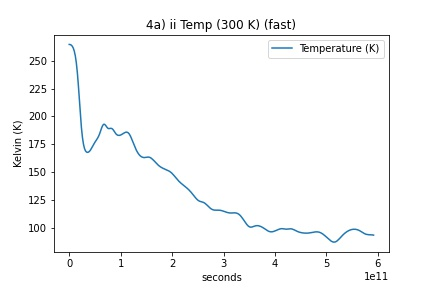
\includegraphics[scale=0.6]{./py/4a_ii_fast.jpg} 
        \caption{108 AR atoms in 27 cells }
        %Label gjør det enkelt å referere til ulike bilder.
        \label{fig:3biv}
\end{figure}

Trying a lower temperature

\subsection*{4a) iii }
\textbf{Find an initial temperature that makes the equilibrium temperature approximately equal to the
94.4 K used in [1]. Plot the temperature as a function of time.
}


We are initializing at 180 Kelvin and getting this result. This is close to the 90 K. 
\begin{figure}[h!]
        \centering 
        %Scale angir størrelsen på bildet. Bildefilen må ligge i samme mappe som tex-filen. 
        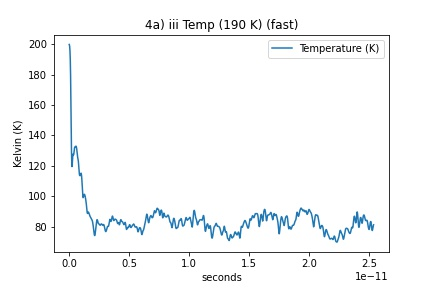
\includegraphics[scale=0.6]{./py/4a_iii_fast.jpg} 
        \caption{4a) iii 108 AR atoms in 27 cells  }
        %Label gjør det enkelt å referere til ulike bilder.
        \label{fig:3biv}
\end{figure}


\subsection*{4b) i}
\textbf{Add the calculation of the velocity autocorrelation to your implementation}

%I have added a function to calculate the velocity autocorrelation.
\newpage
\subsection*{4b) ii}
\textbf{Run a simulation with e.g. 256 atoms (more if you can), and plot the velocity autocorrelation as
a function of time. Compare with figure 4 of the paper}

I have been able t make the following plot with Velocity Autocorrelation \ref{fig:4bii}. Compared to the Landmark study from 1964, the overall exponential fallof is the same, and stabilizing at close to 0 is also similar. However, there are some differences:
\begin{itemize}
\item My Autocorrelation does not fall below 0
\item Characteristic time is not scaled
\end{itemize}

\begin{figure}
\centering
\begin{minipage}{.5\textwidth}
  \centering
  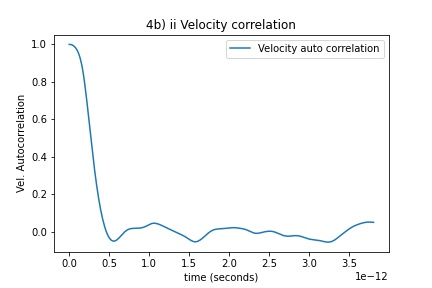
\includegraphics[width=.7\linewidth]{./py/4b_ii_velcorr.jpg} 
  \captionof{figure}{256 AR atoms in 64 cells, starting at 1 }
  \label{fig:test1}
\end{minipage}%
\begin{minipage}{.5\textwidth}
  \centering
  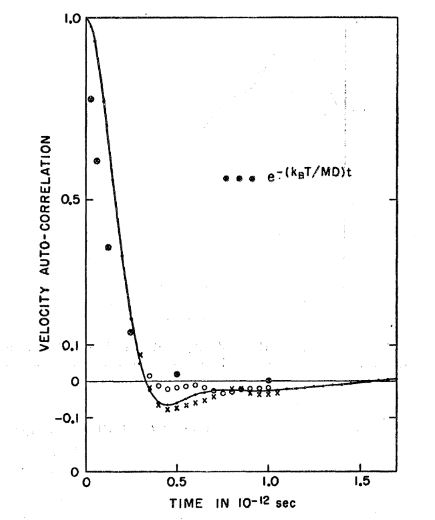
\includegraphics[width=.7\linewidth]{./py/4Rahman.jpg} 
  \captionof{figure}{Plot 4 from Rahman \cite{Rahman 1964}}
  \label{fig:test2}
\end{minipage}
\end{figure}

\newpage
\subsection*{4b) iii}
\textbf{Use the final positions and velocities from the previous simulation as initial positions and
velocities for a new simulation, and calculate and plot the new velocity autocorrelation.}

In this plot we are reading a the last frame of the calculation resulting from task 4b) ii. This allows the chart to begin immediately when the other stops. It looks similar, because what it measures, the correlation with the first frame. There will always be a correlation, and it will always be 1 in the beginning. This is a dimensionsless relation between order and chaos, and is essentially measuring the speed of entropy. For this reason, it looks very similar, even though this autocorrelations is computed from an equillibrium state. 

Plotting the velocity autocorrelation:

\begin{figure}[h!]
        \centering 
        %Scale angir størrelsen på bildet. Bildefilen må ligge i samme mappe som tex-filen. 
        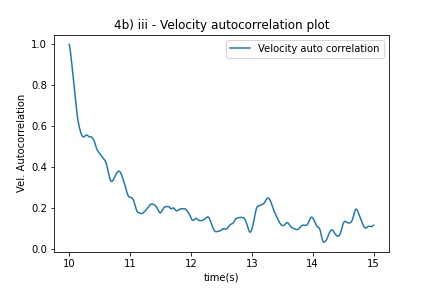
\includegraphics[scale=0.6]{./py/4b_iii.jpg} 
        \caption{ }
        %Label gjør det enkelt å referere til ulike bilder.
        \label{fig:4biii}
\end{figure}


\newpage
\subsection*{4b) iv}
\textbf{If your plot is very noisy (and your program does not run for too long), redo the two abovesimulations multiple times and average the velocity autocorrelation.}

Rerunning the same simulation and averaging over five runs. I've noticed that my potential does not drop below 0, and I am unsure if this is correct or wrong.

\begin{figure}[h!]
        \centering 
        %Scale angir størrelsen på bildet. Bildefilen må ligge i samme mappe som tex-filen. 
        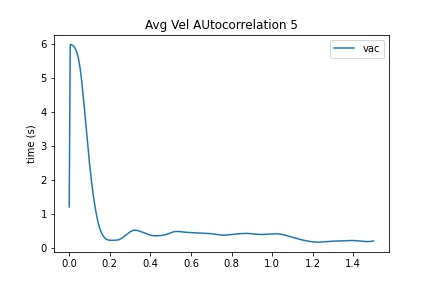
\includegraphics[scale=0.6]{./py/4biv_avg.jpg} 
        \caption{4b iii) 256 AR atoms in 64 cells, averaged over 5 runs}
        %Label gjør det enkelt å referere til ulike bilder.
        \label{fig:4biii}
\end{figure}




\subsection*{4b) v}
\textbf{Estimate the diffusion coefficient from your previously calculated velocity autocorrelation. Compare with the result from [1.}

Diffusion coefficient:

\begin{figure}[h!]
        \centering 
        %Scale angir størrelsen på bildet. Bildefilen må ligge i samme mappe som tex-filen. 
        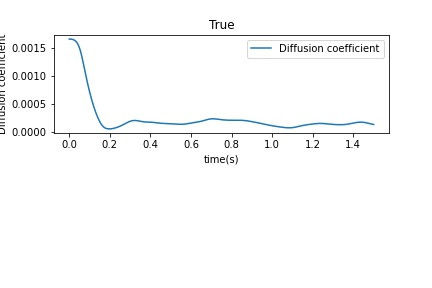
\includegraphics[scale=0.6]{./py/4b_v.jpg} 
        \caption{4b iii) Diffusion coefficient}
        %Label gjør det enkelt å referere til ulike bilder.
        \label{fig:4bv}
\end{figure}

\newpage
\subsection{4c) i}
\textbf{Add the calculation of the mean squared displacement to your implementation}

I decided not to implement counters in all directions, due to the complexity and slowness this imparts on the simulation. Instead, i decided to keep track of another positon vector, the displacement vector which starts at [0,0,0] and the movement is simply added to this in the same way as the x-position, except it never wraps around the periodic boundaries. It does not match the figure from A Rahman at all, probably because my particles remain within bonding reach of each other, i.e the gas is solid, whereas in Rahman the distance covered suggest that it is acting like a gas.

This is an result for four Argon units and 1.5 time.
\begin{figure}[h!]
        \centering 
        %Scale angir størrelsen på bildet. Bildefilen må ligge i samme mappe som tex-filen. 
        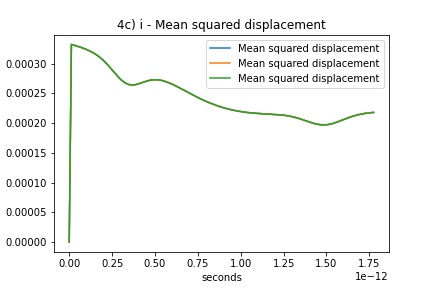
\includegraphics[scale=0.6]{./py/4c_i.jpg} 
        \caption{4b iii) Mean squared displacement}
        %Label gjør det enkelt å referere til ulike bilder.
        \label{fig:4bv}
\end{figure}

\begin{figure}[h!]
        \centering 
        %Scale angir størrelsen på bildet. Bildefilen må ligge i samme mappe som tex-filen. 
        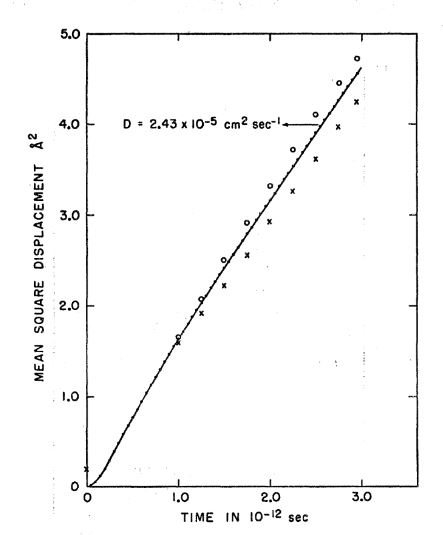
\includegraphics[scale=0.6]{./py/3Rahman.jpg} 
        \caption{4b iii) Mean squared displacement }
        %Label gjør det enkelt å referere til ulike bilder.
        \label{fig:4bv}
\end{figure}

\newpage
\subsection{4c) ii}
\textbf{Implement the calculation of the diffusion constant, and run a simulation for 864 atoms (fewer
is also fine if the runtime is slow). How does your result compare to the one in [1]?
}

Calculating the diffusion constant. It is not possible to compare a chart of th diffusion constans, as there is no such chart in the paper of A. Rahman. 

\begin{figure}[h!]
        \centering 
        %Scale angir størrelsen på bildet. Bildefilen må ligge i samme mappe som tex-filen. 
        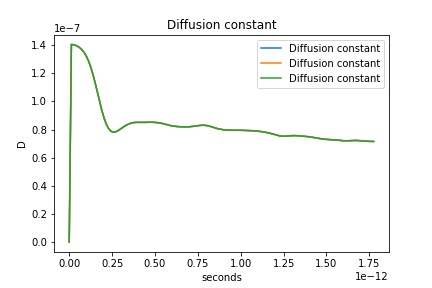
\includegraphics[scale=0.6]{./py/4c_ii_diffusionConstant.jpg} 
        \caption{4c ii) Diffusion constant }
        %Label gjør det enkelt å referere til ulike bilder.
        \label{fig:4cii_diffusionconstant}
\end{figure}

\subsection{4d) i}
\textbf{Run a simulation with as many atoms for as long as you can. Calculate the radial distribution
function g(r), plot the result and compare with figure 2 of [1].}

We use 12 bins, and bin the atoms in a histogram based on their distance form each other. Simulation are initialized at 190 Kelvin, time is given by  $ $seconds for 864 particles. 

I am not able to reproduce the sinusoid probability density in Rahmans paper. It is possible, that this is due to the high number of particles and a relatively small box. With 864 particles and a $15^3 \sigma$ enclosure, each particle has only $3.95 \sigma^3$ of space, putting the mean distance between particles at $3.95 \sigma$. This will skew the distribution toward the left, possibly explaining the deviation from Rahman.




\begin{figure}[h!]
        \centering 
        %Scale angir størrelsen på bildet. Bildefilen må ligge i samme mappe som tex-filen. 
        
\includegraphics[scale=0.6]{./py/4di_rdf_bar.jpg} 
        \caption{4d) i : Counts for bins.  }
        %Label gjør det enkelt å referere til ulike bilder.
        \label{fig:4di_rdf_plot}
\end{figure}


\begin{figure}[h!]
        \centering 
        %Scale angir størrelsen på bildet. Bildefilen må ligge i samme mappe som tex-filen. 
        
\includegraphics[scale=0.6]{./py/4di_rdf_plot.jpg} 
        \caption{4d) i : Radial distribution function plot }
        %Label gjør det enkelt å referere til ulike bilder.
        \label{fig:4di_rdf_plot}
\end{figure}

\begin{figure}[h!]
        \centering 
        %Scale angir størrelsen på bildet. Bildefilen må ligge i samme mappe som tex-filen. 
        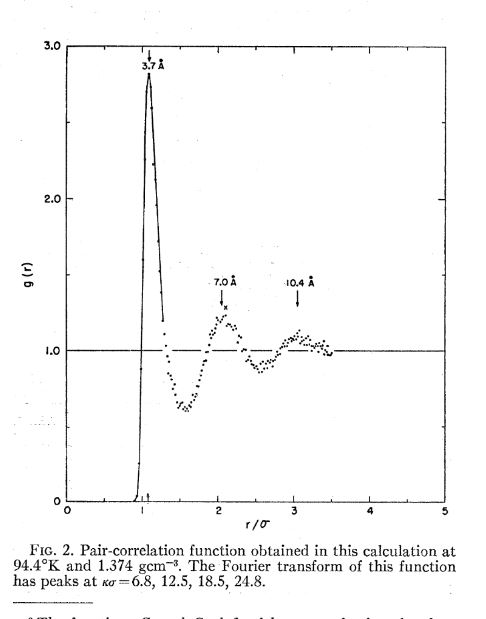
\includegraphics[scale=0.6]{./py/Rahman2.jpg} 
        \caption{4d) i : Rahman fig 2 }
        %Label gjør det enkelt å referere til ulike bilder.
        \label{fig:Rahman2}
\end{figure}

Python code is available as zip file.

\end{document}
